\section{分量旋转}
\label{sec:traces-rotating}
相关命令:\nameref{cmd:rotate}

相关头段:cmpinc、cmpaz

三个正交的地震传感器即可完全记录地面运动矢量。因此可以将三个正交的分量任意旋转
到其它三个正交的方向上。

出于仪器安装的考虑,地震仪三分量一般都是N、E、U向的。而地震学里,由于
SH波与P-SV波的解偶,更常处理的是R、T、Z向的三分量数据。因而地震信号的旋转是有
必要的。

SAC提供了rotate命令,用于旋转任意两个分量。在旋转之前,SAC会检查两个分量的cmpinc
和cmpaz,确定二者是正交的。

\begin{SACCode}
SAC> dg sub teleseis ntkl.[enz]
/opt/sac/aux/datagen/teleseis/ntkl.e ...ntkl.n ...ntkl.z
SAC> w ntkl.e ntkl.n ntkl.z
SAC> r ./ntkl.n ./ntkl.e
SAC> lh cmpinc cmpaz
  
  FILE: ./ntkl.n - 1
 --------------

     cmpinc = 9.000000e+01
      cmpaz = 0.000000e+00
  
  FILE: ./ntkl.e - 2
 --------------

     cmpinc = 9.000000e+01
      cmpaz = 9.000000e+01
SAC> rotate to gcp              // 旋转到大圆路径
SAC> lh cmpinc cmpaz
  
  FILE: ./ntkl.n - 1
 --------------

     cmpinc = 9.000000e+01
      cmpaz = 2.440466e+01
  
  FILE: ./ntkl.e - 2
 --------------

     cmpinc = 9.000000e+01
      cmpaz = 1.144047e+02
SAC> w ntkl.r ntkl.t            // 保存为R分量和T分量
\end{SACCode}

图~\ref{fig:rotate}~中,左图中从上至下为N、E、Z分量,右图中从上至下为R、T、Z分量。
旋转到R、T分量后,可以很容易地识别出Rayleigh和Love波。

\begin{figure}[H]
\centering
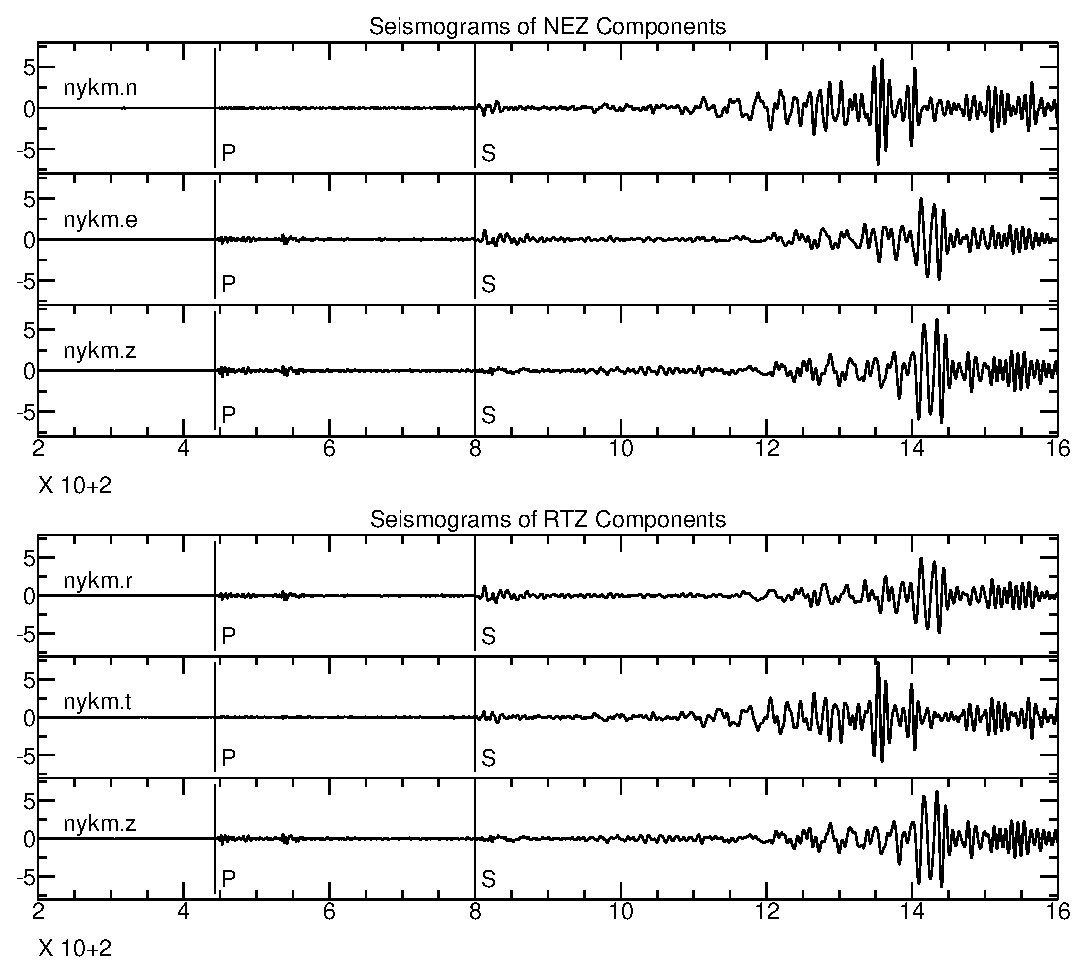
\includegraphics[width=0.95\textwidth]{rotate}
\caption[水平分量旋转]{将N、E分量旋转到R、T分量。}
\label{fig:rotate}
\end{figure}
